%
\documentclass[runningheads]{llncs}
%
\usepackage{graphicx}
% Used for displaying a sample figure. If possible, figure files should
% be included in EPS format.
%
% If you use the hyperref package, please uncomment the following line
% to display URLs in blue roman font according to Springer's eBook style:
% \renewcommand\UrlFont{\color{blue}\rmfamily}

\title{A CNN Based AMOLED Display Aging Compensation Quality Evaluation System\\
ECE657A Spring2020 Project Report}
\author{Alyssa Yiqin Huang, Tong Liu}
\date{15th ,August 2020}

\institute{Electrical and Computer Engineering, University of Waterloo\\
200 University Ave W, Waterloo, ON N2L 3G1, Ontario, Canada\\
\email{ yiqin.huang@uwaterloo.ca ,t344liu@uwaterloo.ca}}
\begin{document}

\maketitle              % typeset the header of the contribution
%
\begin{abstract}
An accurate and quick display luminance uniformity evaluation function plays a key feedback role for the automated AMOLED Display aging compensation evaluation system. In this report we discuss a CNN autoencoder based luminance uniformity evaluation system which we designed and implemented for AMOLED display aging compensation performance evaluation. Within a short period of time we are able to design, implement the system and use the system to detect whether an aged AMOLED display has a high quality compensation, a low quality compensation or had no compensation in a relatively good accuracy rate.

\keywords{ CNN autoencoder\and Active Matrix OLED - AMOLED\and AMOLED Display Aging\and AMOLED Display Aging Compensation \and Luminance Uniformity}
\end{abstract}

%
%
%
\section{Introduction}
AMOLED display panel has been widely used as high-end smart phone display, TV display and
automotive car informatic display. A major long-term performance issue of AMOLED display is OLED
material aging, which is the luminance performance drop at aged area cause nonuniformity issue on AMOLED display. This luminance nonuniformity shows a symptom is called burn-in see \ref{fig:1}.
To solve OLED aging issue and eliminate burn-in on AMOLED display, Ignis Innovation Inc. has developed a state of art OLED aging compensation solution to solve OLED aging problem see \ref{fig:2}.
However, to evaluate the OLED aging compensation quality is processed based on human vision. It
takes a lot of time. Its evaluations vary from person to person and difficult to compare between
evaluation results. How to evaluate the quality of OLED aging compensation with a speedy and
accurate approach is a technical challenge.
During ECE657A project, we tried to develop an OLED aging compensation evaluation function to solve above technical challenge by using the knowledge and techniques which we have learned in this course. We build a prototype system which is having conceptual functionality works as expect. The system able to detect the AMOLED display OLED aging compensation quality is GOOD or BAD. GOOD compensation quality means with OLED aging compensation, the brightness uniformity on the OLED display is beyond a certain threshold. Apparently, there will be no visible burn-in aging area on display while smart phone is normally running.BAD compensation quality means with OLED aging compensation the brightness uniformity on the OLED display is below to a certain threshold. There could be some visible burn-in area still showing on OLED display

\begin{figure}
    \centering
    \subfigure[a]{
        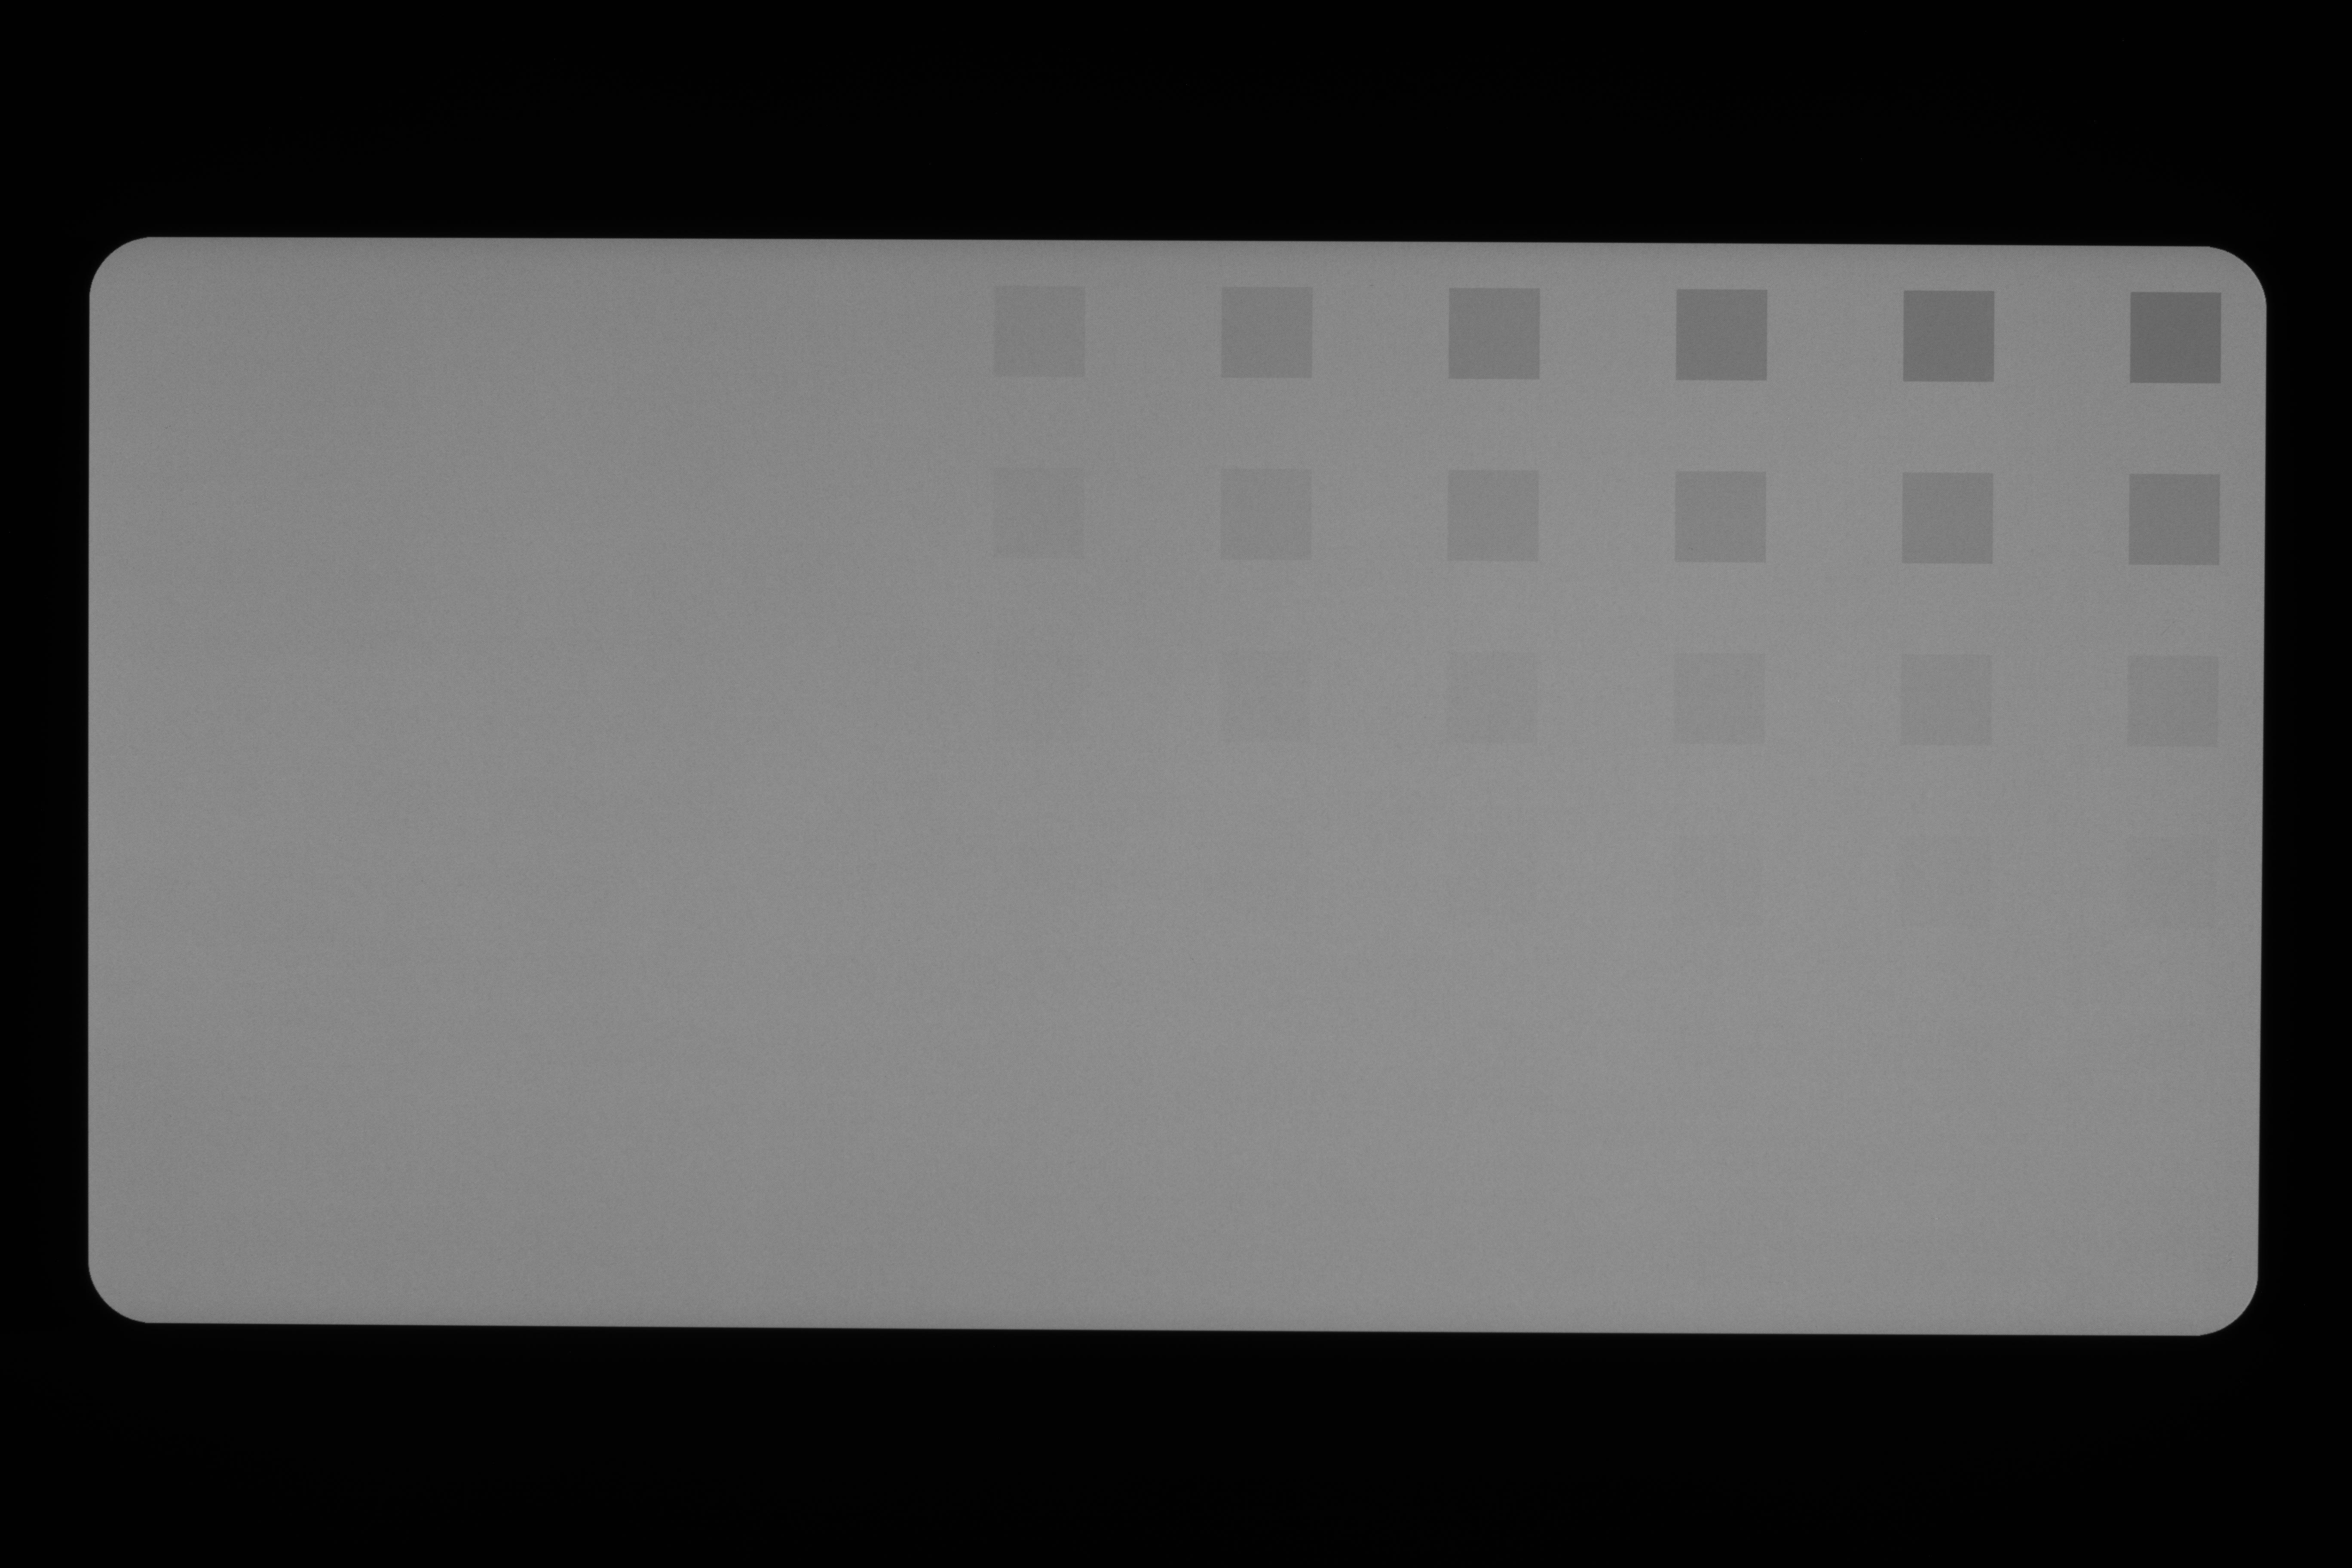
\includegraphics[width=0.4\textwidth]{uncomp.jpeg}}
   \subfigure[b]{
        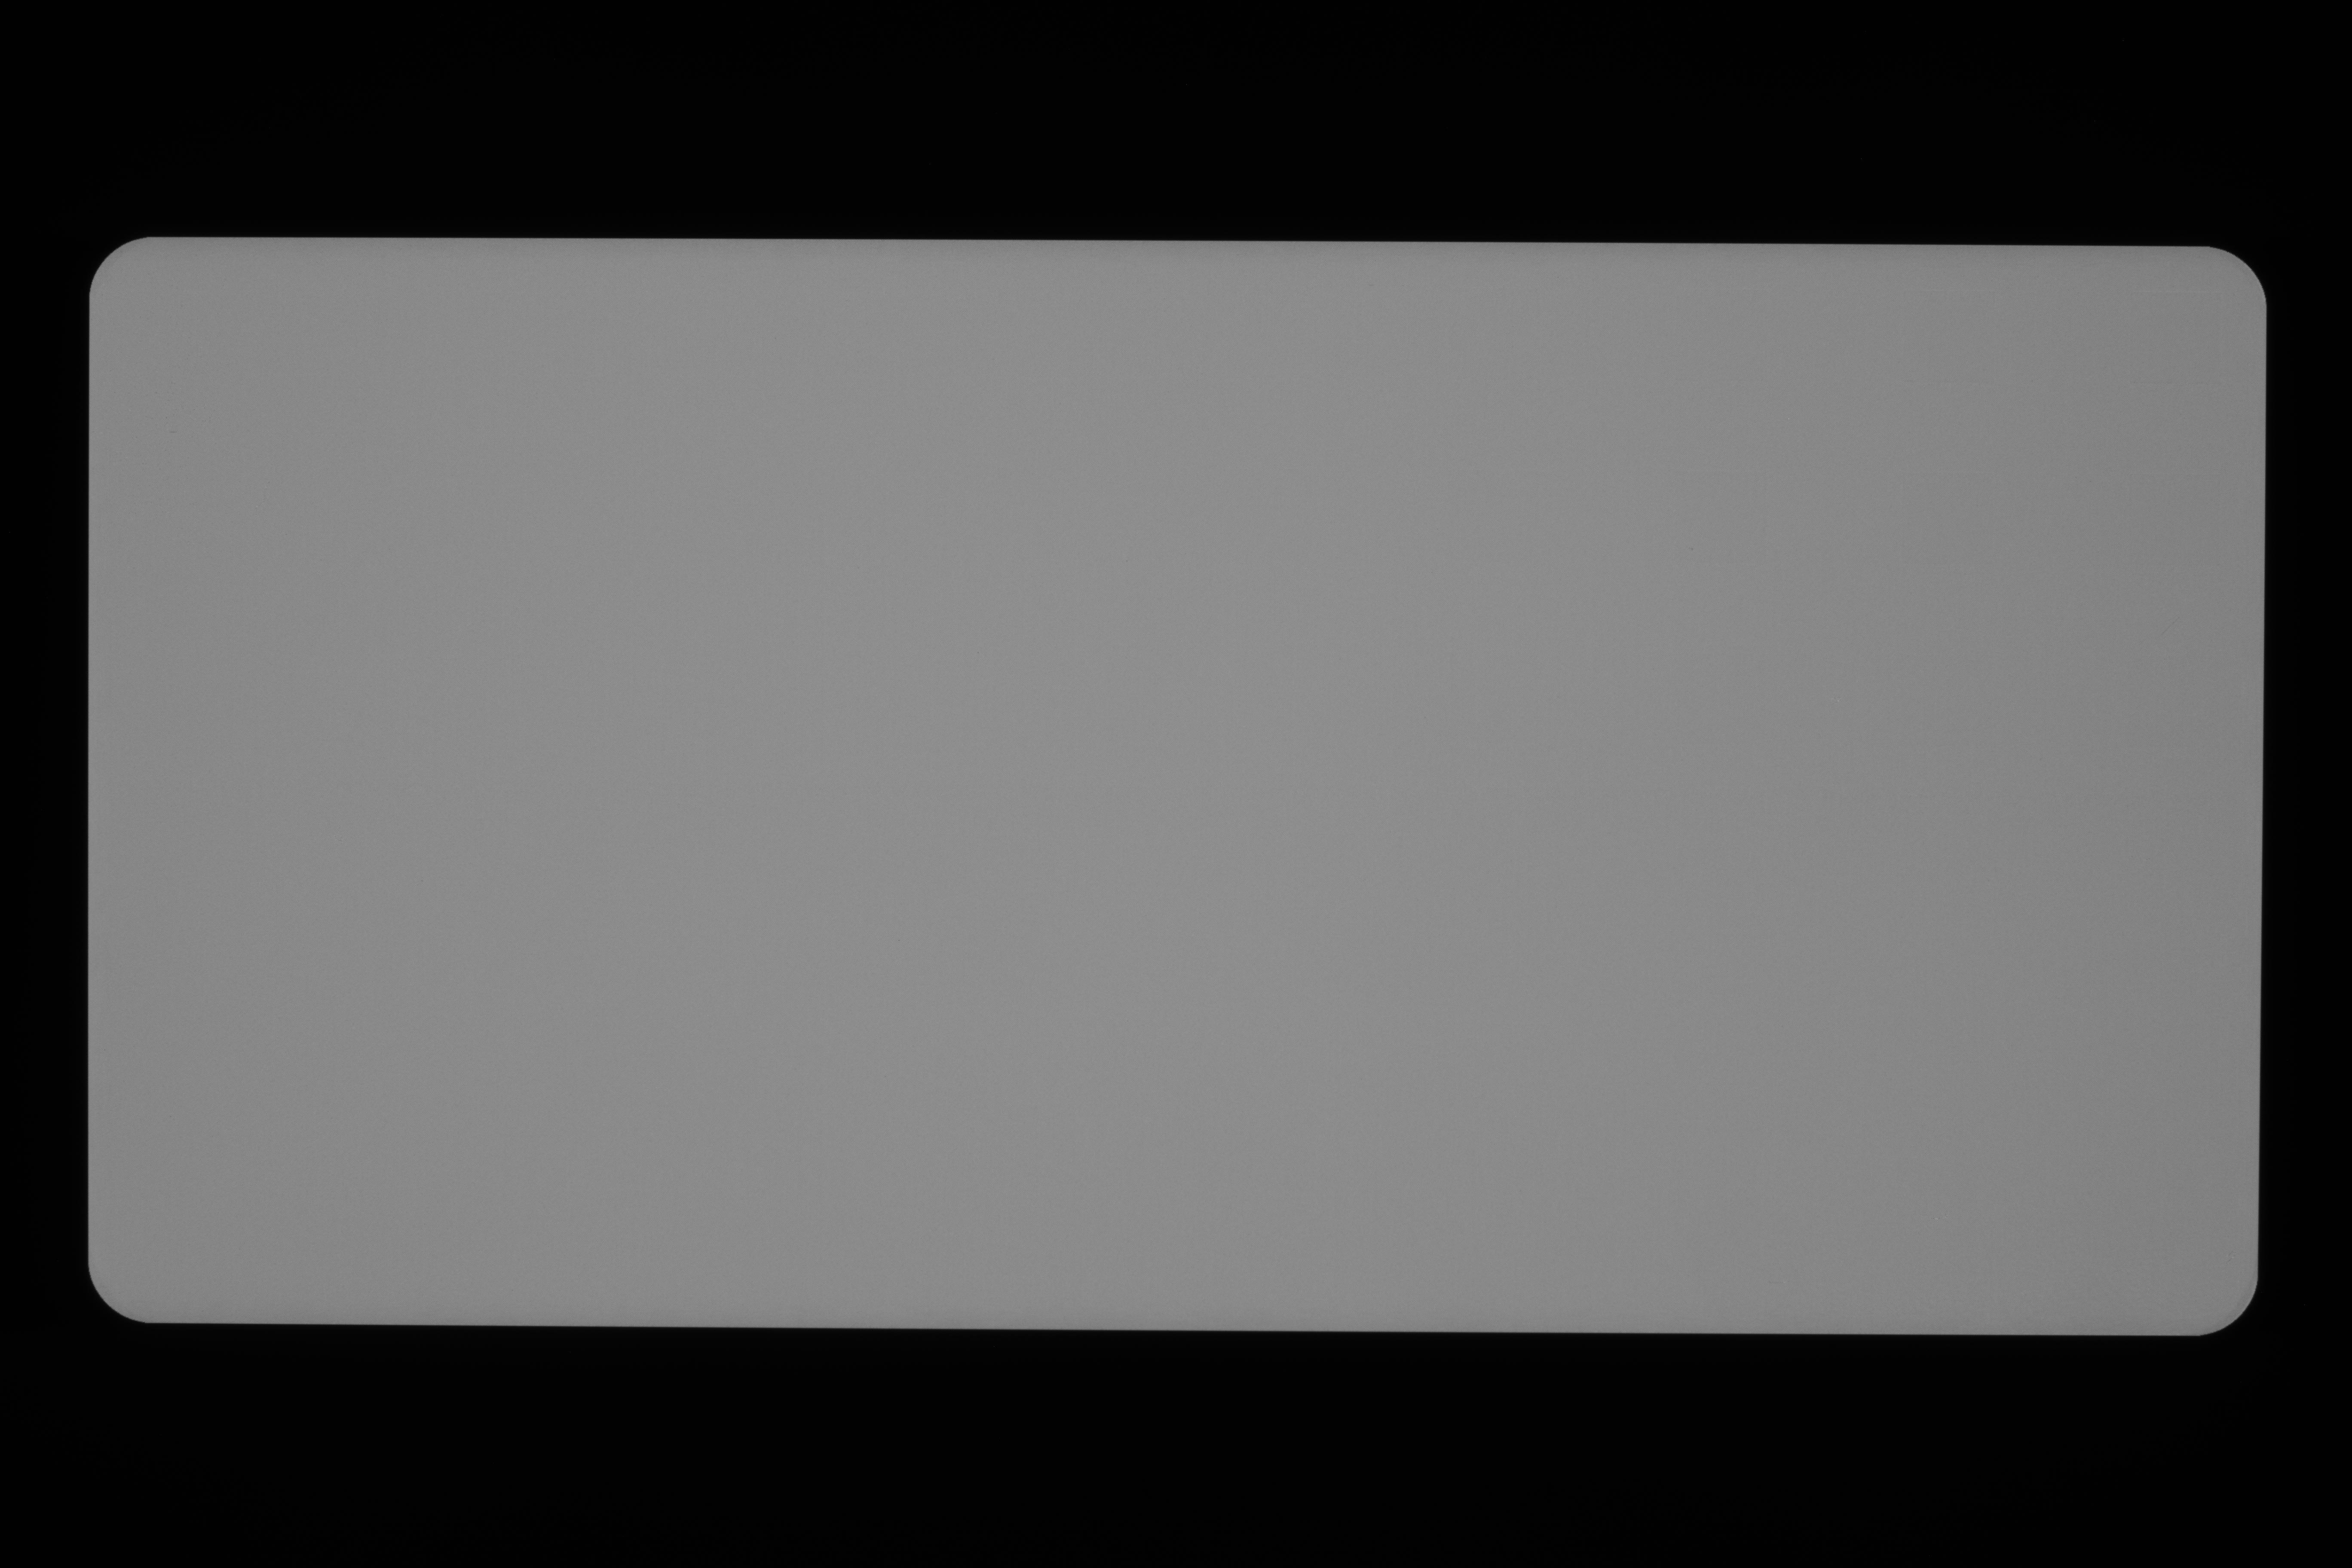
\includegraphics[width=0.4\textwidth]{comp.jpeg}}
    \caption{ (a) An Aged AMOLED display (b)With OLED aging compensation,the same AMOLED display's burn-in is eliminated }        
    \label{fig:1}
\end{figure}

\section{Literature review}
In order to archive the project, except the materials we learned from ECE657A course, we also referenced a numbers of papers in the fields of image processing, machine learning ,deep learning and AMOLED display technologies. 
Peter Barten’s research on the contrast sensitivity of human eye [10] provides a formula for contrast sensitivity which is helpful to improve accuracy of result by minimize the contrast sensitivity various of human eye. This can be done by implementing contrast sensitivity function to emphasis the difference between AMOLED display's normal areas and OLED aging areas.
Kazuki Tsutsukawa and his team at EIZO Corporation, developed an Evaluation system for Luminance Non-Uniformity Based on Deep Neural Networks. Their research paper shows that the possibility for using deep neural networks [4] to evaluate luminance non-uniformity automatically, which enables optimization of feature quantity extraction.

\section{Design Considerations}
\begin{figure}
    \centering
    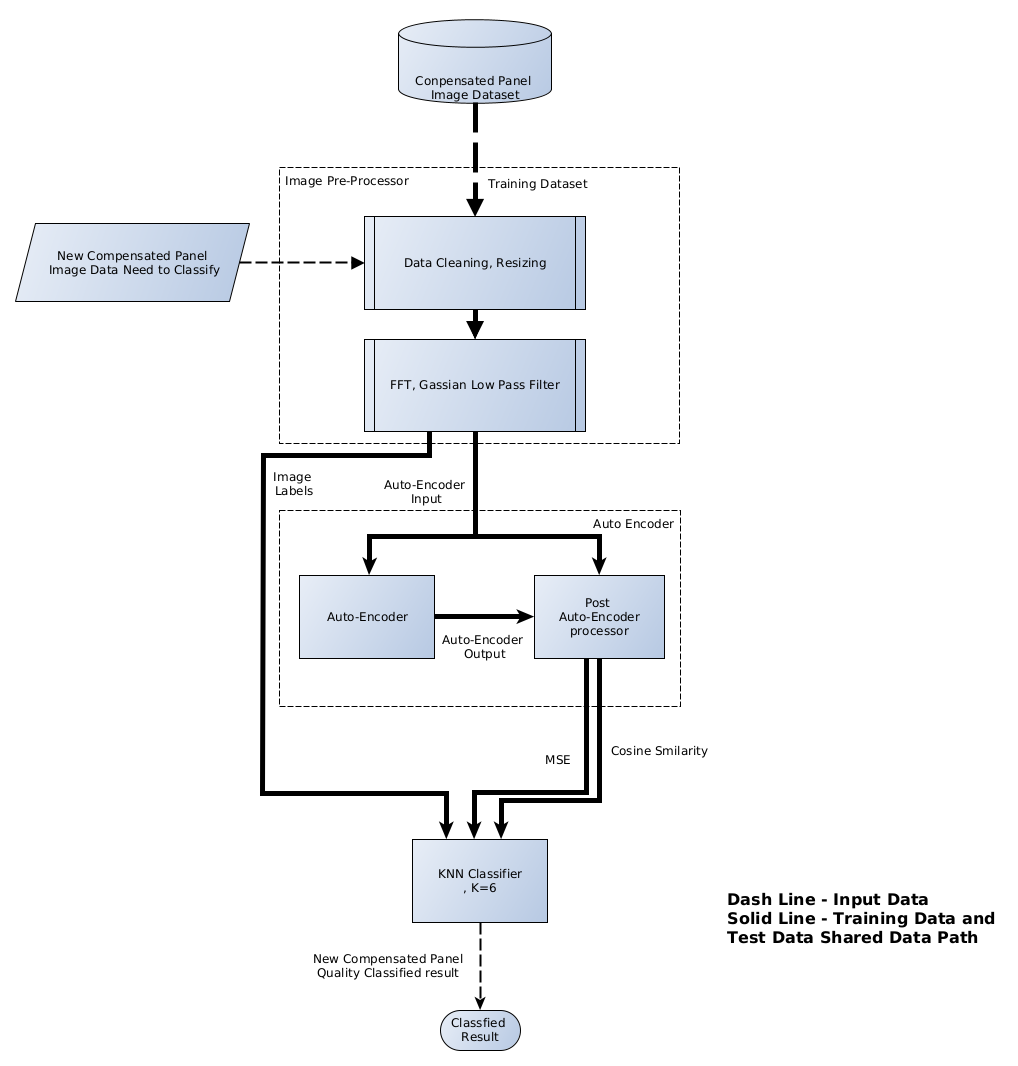
\includegraphics[width=1.0\textwidth]{system-diagram.png}
    \caption{System Design Diagram}
    \label{fig:2}
\end{figure}
We design the system under below considerations. Figure\ref{fig:2} shows a high level overall system diagram of our system. We will briefly discuss each part of the system in this section.

\subsection{System Input - Load Training Dataset}
System shall take image files from specified folder which contains two sub-folders - "good" and "bad". They stores the panel image files. Folder "good" contains panel images those have good quality compensation, folder "bad" contains panel images those have bad quality of compensation. The image file shall be either jpeg or png format. System will use these data folders as training datasets, the folder names "good" and "bad" will be used later in the project as label.
\subsection{Data Pre-process}
After images were loaded, these images need to be pre-processed in order to fit into system to train system. We need to perform following steps as data pre-processing.
\item{a, Preform image data integrity check}
\item{b, Data cleaning}
\item{c, Resizing the image to meet the quality and speed requirements}
\item{d, Run selected image filter to emphasis image's the non-uniform area}\\
We will discuss details in "System Implementation" section\\
\subsection{Auto-Encoder}
Alyssa put more details\\
The auto-encoder takes pre-processed image data as input data fit into auto-encoder, get auto-encoder's output data. Based on auto-encoder's input and output data calculate two indicators as 2 dimensional result. 
First indicator is Mean square error of input and output data. The second indicator is Cosine similarity of input and output data. \\
\subsection{Find System Decision Boundary}
We will use a set of pre-classified labeled panel image data which were taken in the past as dataset to train system. After entire dataset went through auto-encoder, we shall get two dimensional data arrays of MSE and Cosine similarity, fit this 2D data array with "good/bad" label information to a classifier, then we shall be able to find good/bad compensation quality decision boundary. 
\subsection{System Output}
Once system and classifier was trained, the system is ready to take testing set to detect whether the display panel had a good or bad quality compensation.

\section{System Implementation}
Based on the design considerations those we discussed in previous section, we implemented the system with python. Here we will discuss more implementation details in this section. 
\subsection{Image pre-processing}
Image pre-processor plays an important role in this system. As sample image loaded from dataset has to meet the requirements of autoencoder to archive the goal, and meet the quality and speed performance requirements.  We have implemented numbers of pre-process functionalities mainly in two parts. \\
\begin{figure}
    \centering
    \subfigure[a]{
        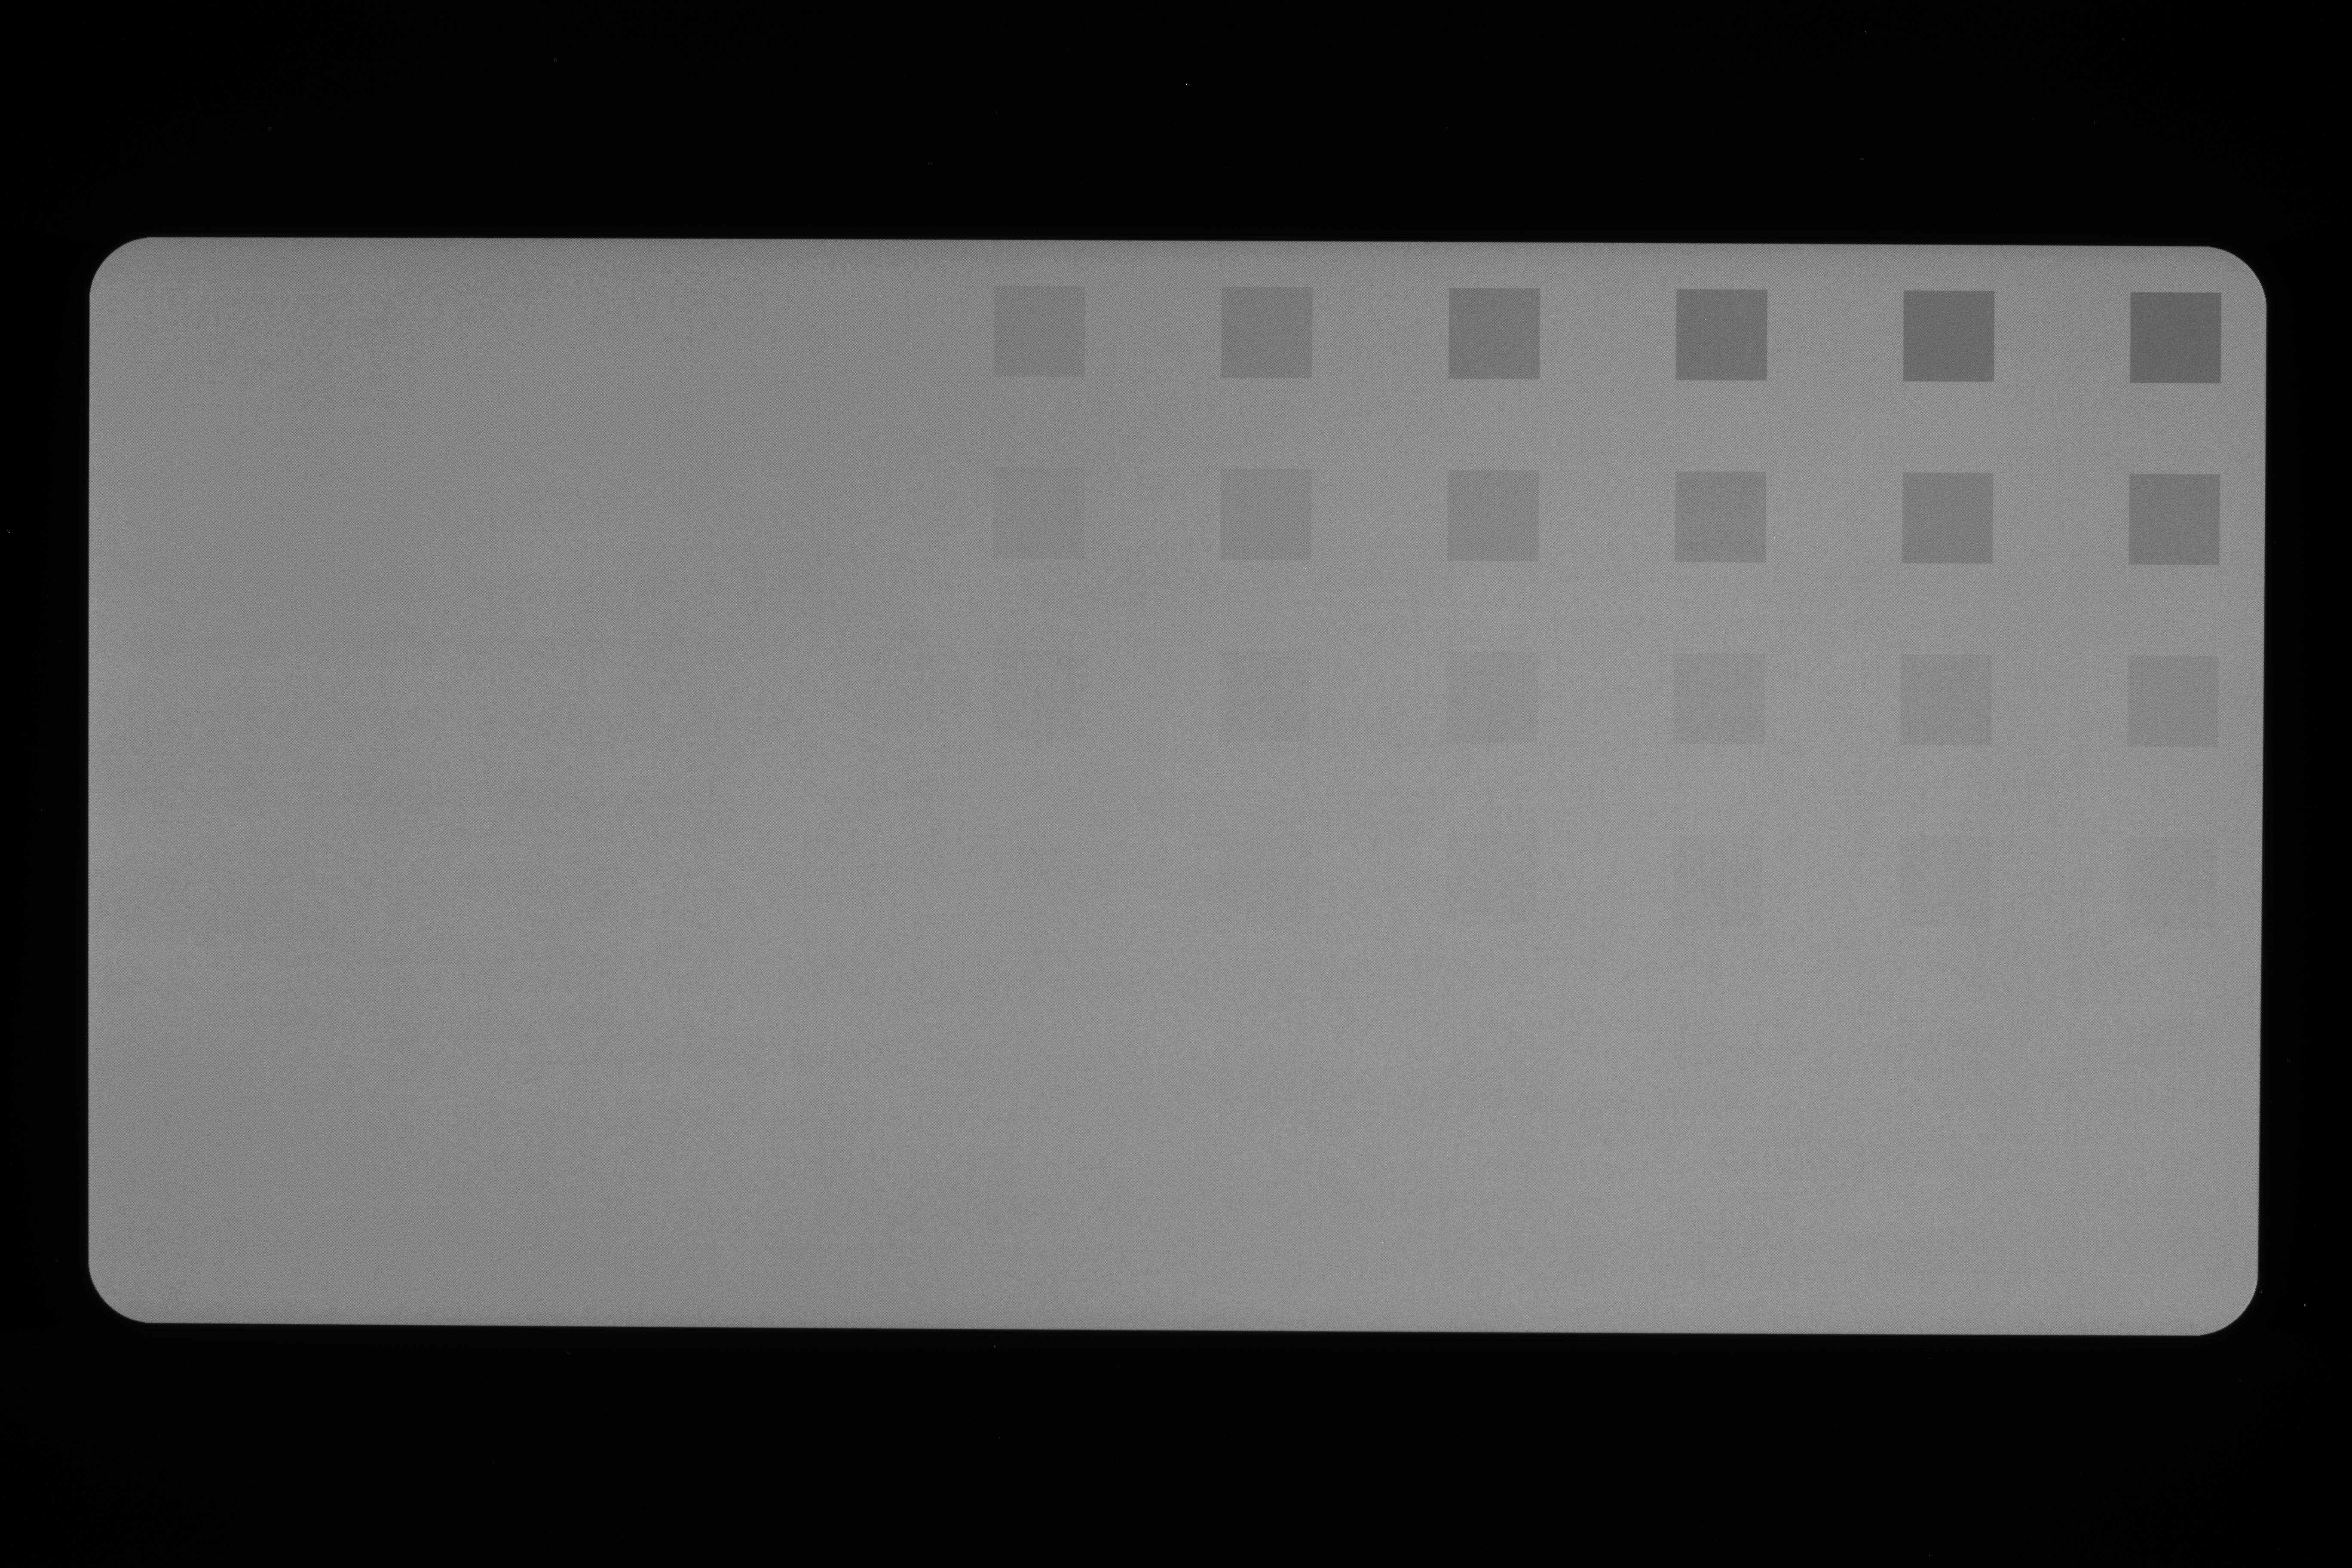
\includegraphics[width=0.4\textwidth]{Pixel2-uncomp-original.jpeg}}
   \subfigure[b]{
        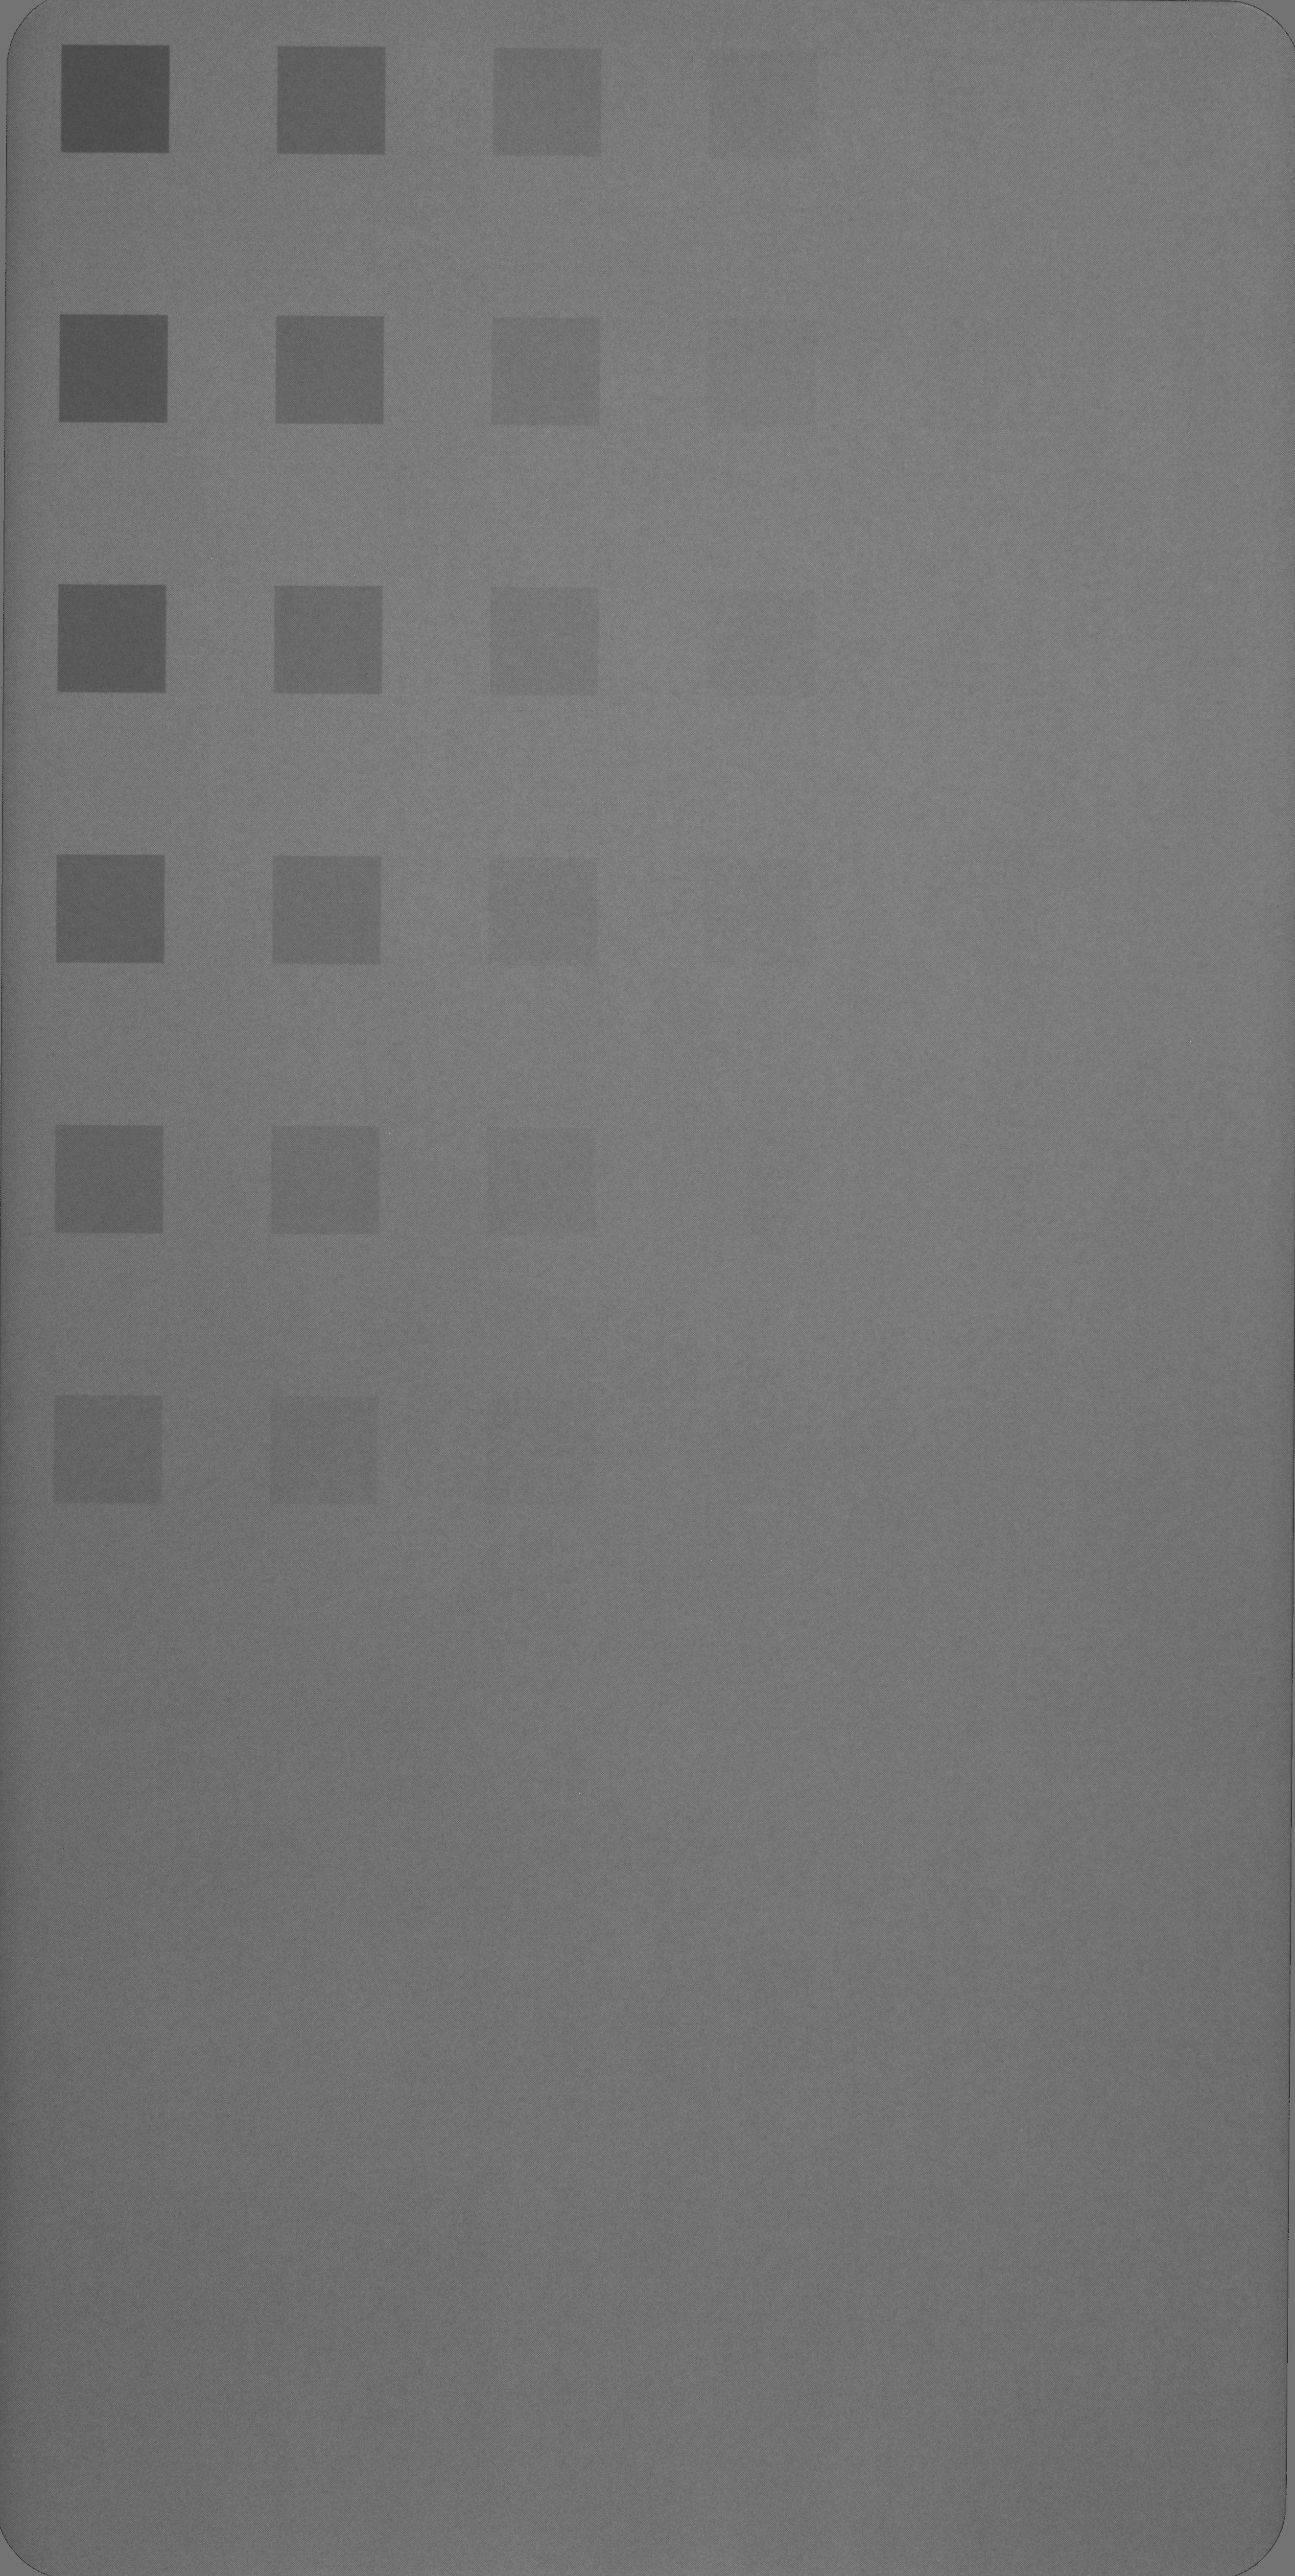
\includegraphics[width=0.2\textwidth]{Pixel2-Uncomp-g.jpeg}}
    \caption{ (a) Original panel Image (b)Panel Image After Data Cleaning }        
    \label{fig:3}
\end{figure}

First part includes data cleaning, data resizing, data flatten, and etc. Figure\ref{fig:3} shows AMOLED panel image before and after data cleaning process. In original image there are dark areas were taken by camera, they need to be cut, and dark areas at four corners need to be cleaned by filled with mean value.\\
\begin{figure}
    \centering
    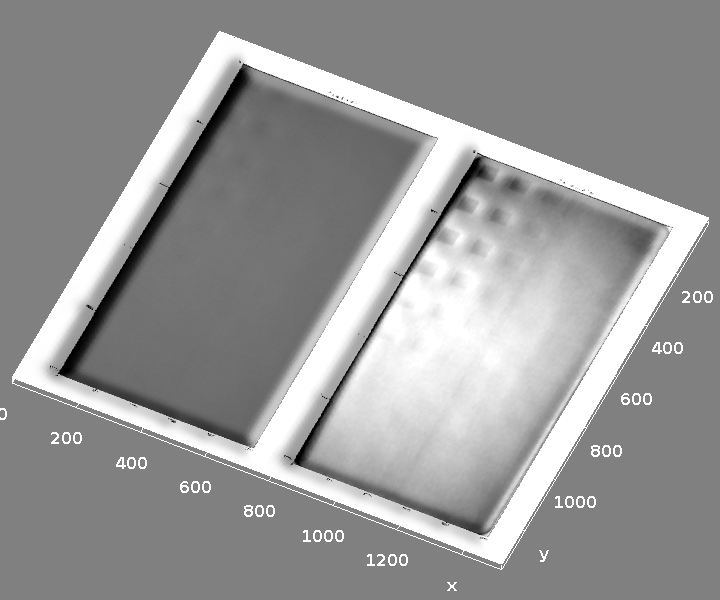
\includegraphics[width=0.8\textwidth]{Surface_Plot_of_3D_plot_resized_fft_lowpass.png}
    \caption{Image Data before and after FFT Gaussian Low Pass Filter}
    \label{fig:4}
\end{figure}
The second part of image pre-processing is image data filtering process. \\
In our project proposal, we mentioned we planned to implement a CSF - Contrast Sensitivity Function, to reduce impact by the difference of sensitivity between each human eyes. However, while we are working on implementation we noticed that to be able to calculate the contrast sensitivity, we need four parameters, they are spatial frequency in cycle/degree, display luminance, surround luminance, Field of view in degree, we realized that we were lacking the equipment to measure surround area luminance data during the panel measurement. As the trade off, we decided to use FFT-Gaussian-LowPass filter to enhance the luminance difference between the nonuniform and uniform areas of AMOLED panels. The output from FFT-Gaussian-LowPass filter is used as Auto-encoder's input. \\

Figure\ref{fig:4} shows that the pre-processed original image and the image after FFT-Gaussian-Lowpass filter processed. The image in this figure was a taken from a panel which had applied OLED compensation on the panel, however, the compensation wasn't perfect, as we still able to see little Burn-in on the panel, even them were not obvious, please see the left side of figure\ref{fig:4}. At here, let's compare the left side of plot with the right side of plot, we can clearly see that after FFT-Gaussian-Lowpass filter processing, luminance difference between the compensated area and normal areas was emphasized by the filter.
After image pre-processing phase, the pre-processed data will be passed to next major module - the CNN based auto-encoder. 
\subsection{CNN based Auto-encoder}

\subsection{Choose Classifier and Decision Boundary}
From auto-encoder, we get two sets of compensation quality evaluation indicators. MSE and Cosine Similarity. The next step is use these indicators and image sample label to train classifier, Classifier is trained with training dataset, after training the system is ready for the AMOLED aging compensation quality classification.\\
\begin{figure}
    \centering
    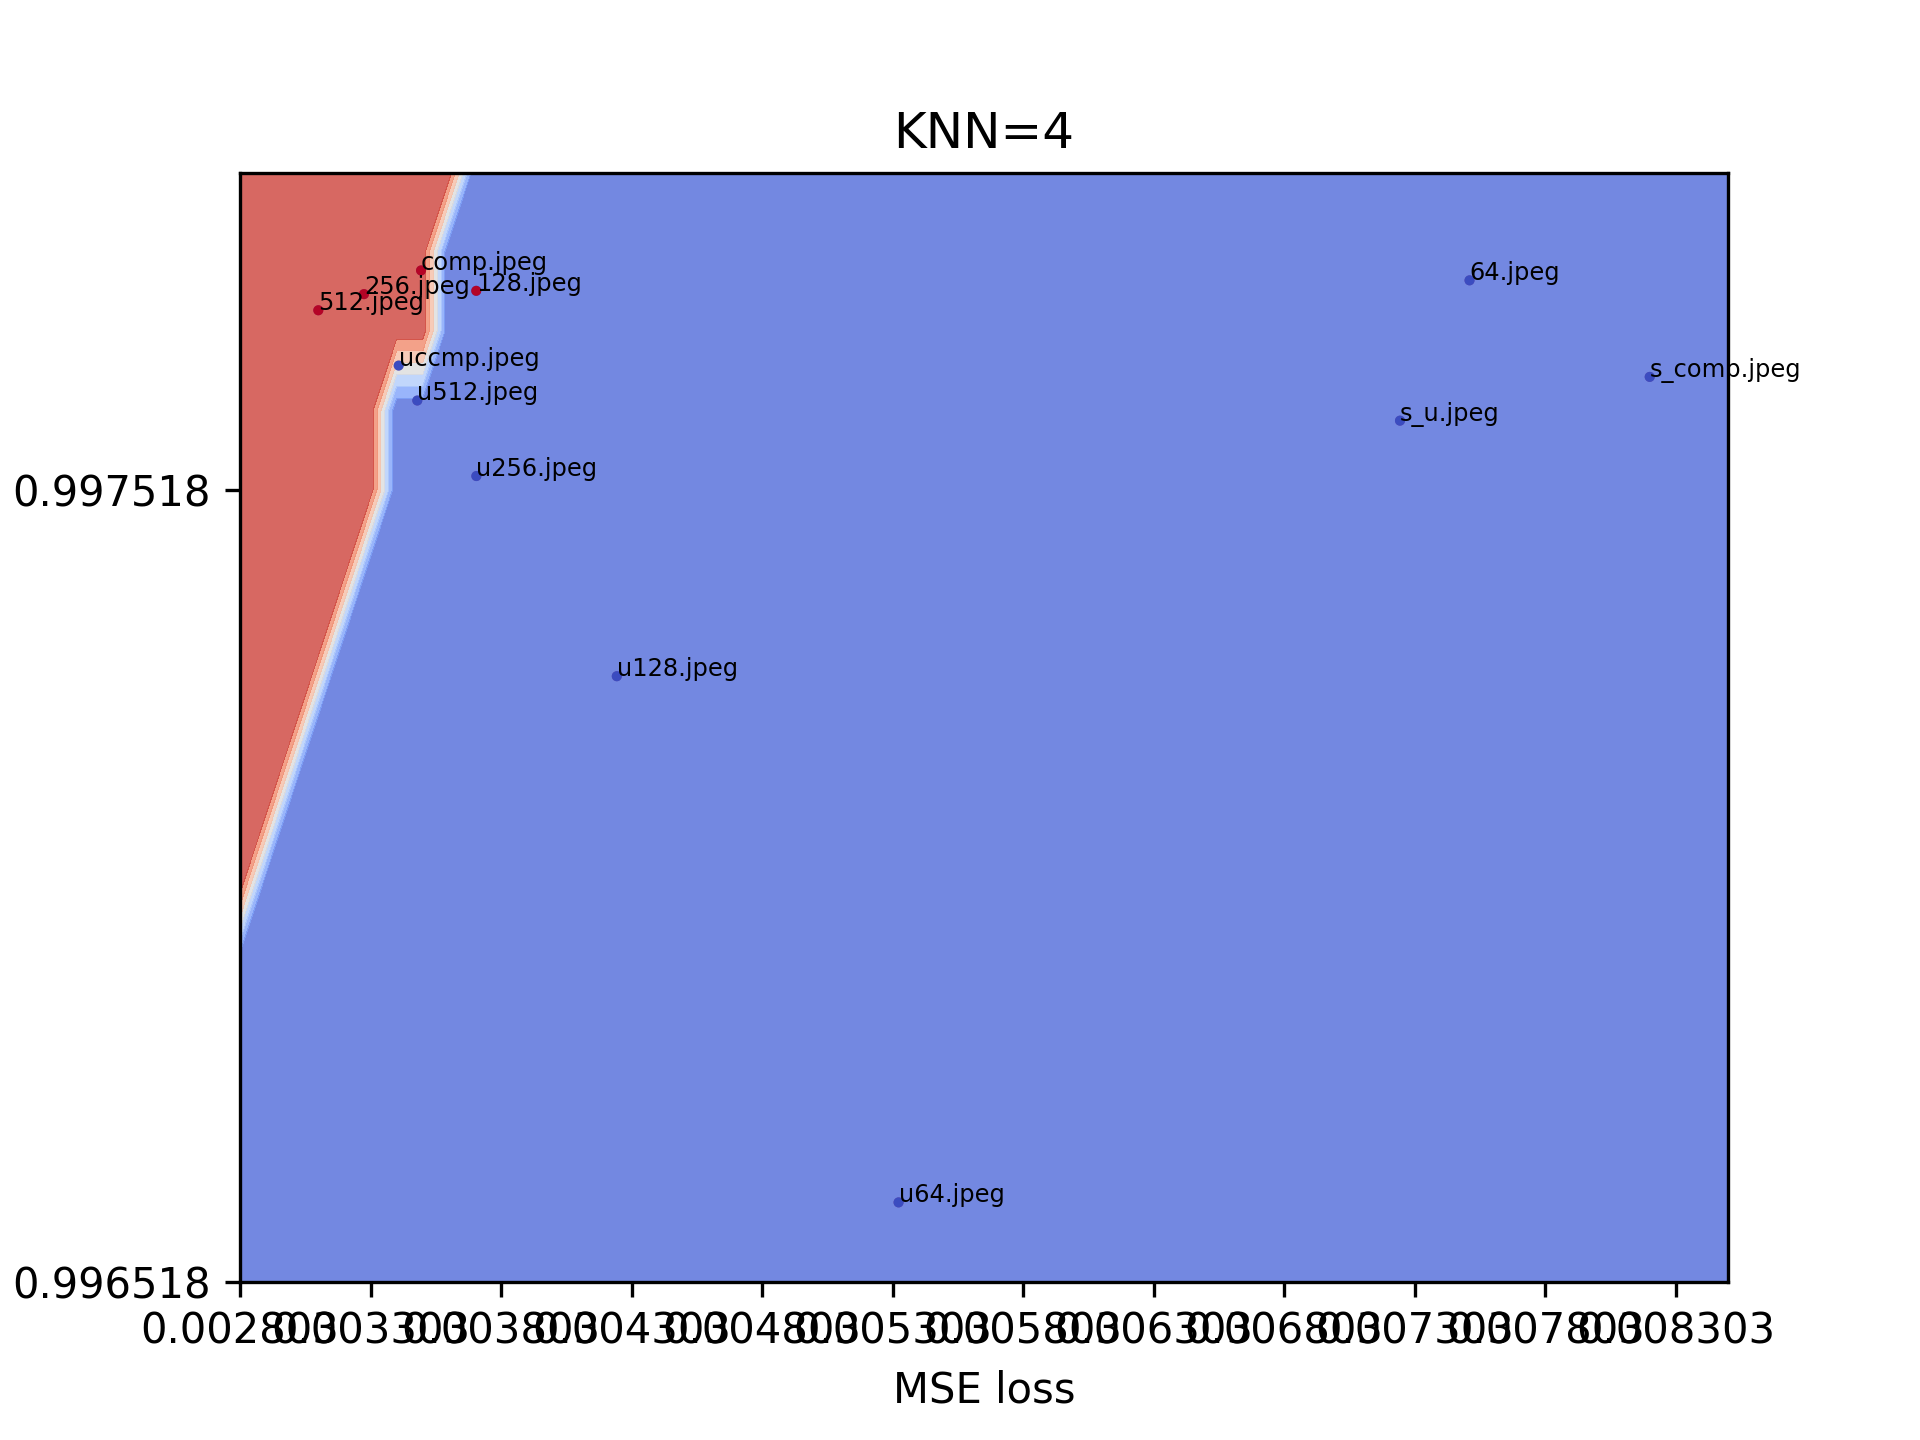
\includegraphics[width=1.2\textwidth]{decision-boundary.png}
    \caption{Decision Boundary}
    \label{fig:5}
\end{figure}
Due to the limited samples, it gave us some difficulty to choose a classifier with better performance, and clear decision boundary. We took some time to work on choosing suitable classifier for this project. Based on current image samples, finally we chose KNN as classifier with K equal to 6. Please see figure\ref{fig:5} which shows comparsion of decision boundary based on training samples. As we can see the KNN algorithm shows clearest boundary than others, some of the algorithm even couldn't find a decision boundary under the same condition as KNN has. The decision boundary plot based on two performance indicators. The Y axis is Cosine similarity, and X Axis is Mean Square Error, any image sample fall into the Left-Upper corner of the plot indicates the high compensation quality, on the other side indicates bad compensation quality.\\

In the future as we could get more image samples, we would redo the evaluation for the classifier selection, and then we could have more accurate decision boundary based on larger dataset as compensation quality selection base.

\section{Testing and Results}
Once decided to use KNN classifier with K equal to 6,  we validated system with following procedure. 
We use total 87 panel images as trainig dataset, and take aother 22 panel images as test dataset. These panel images were pre-classified and labeled manually in the previous work. Both training dataset and test dataset ran through the pre-processing and auto-encoder, then we got MSE and Cosine similarity sets for training datseta and test dataset. Fit training dataset MSE/Cosine Similarity to KNN classifier first, then fit test dataset's MSE/Cosine Similarity to KNN classifier to get predicted result. \\
Finally we got confusion matrix as table\ref{tab:cm}, based on confusion matrix we calculated classifier accuracy wsa 95.5\%, and classifier precision was 96.7\%\\
\begin{table}
    \centering
    \caption{Classifier Confusion Matrix}
    \label{tab:cm}
\begin{tabular}{cc}
    & Actual \\
    Predicted & $\begin{bmatrix}\ 
        14 & 0 \\
        1 & 7\\
        \end{bmatrix}$\\
\end{tabular}
\end{table}
\section{Discussion}
How to evaluate the quality of compensation of AMOLED display panel in an accurate and fast way, is technique challenge. As a experiment, we ran a pure classification process with SVM with linear and RBF kernel.  
Both svm kernels brought us lower accuracy about 57.1\% and 65.2\%
This shows that difficulty of catch and evaluate the luminance difference accurately between good and bad compensation. Because of that, using a pure classic classifier like SVM to evaluate panel image luminnance uniformity couldn't bring us accurate result.\\
Our approach is focus on emphasis the lunminance differences by using FFT-Gaussian-lowpass filter, and furthermore, using a convolution neural network based auto-encoder, to enlarged difference between input and output.
At end calculate two indicators MSE and Cosine similarity, and use them to identify the image quality class to give us better accuracy for about 96.7\% .
\section{Conclusion and Future work}


\section{Reference}
\end{document}

